\documentclass[conference]{IEEEtran}
\usepackage{cite}
\usepackage{amsmath,amssymb,amsfonts}
\usepackage{algorithmic}
\usepackage{graphicx}
\usepackage{tabularx}
\usepackage{color}
\usepackage{fancyvrb}
\usepackage{fvextra}
\usepackage{float}
\usepackage[table]{xcolor}
\usepackage{tcolorbox}
\usepackage{listings}
\usepackage{cuted}
\usepackage{xcolor}
\usepackage{appendix}
\usepackage{amsmath}
\usepackage{amssymb}
\usepackage{algorithmicx}
\usepackage[noend]{algpseudocode} 

\definecolor{lightgray}{rgb}{0.95,0.95,0.95}
\lstset{
    language=Python, 
    basicstyle=\ttfamily\footnotesize,
    breaklines=true, 
    frame=single,
    showstringspaces=false,
    backgroundcolor=\color{lightgray},    
    captionpos=b
}

\begin{document}

%\title{Integrating Generative AI into Mobile Networking}
\title{An LLM Reasoning Framework for Automatic gNB Parameter Adjustment Using Synthetic Training Data}
\author{\IEEEauthorblockN{
        Yao-Cong Dong\IEEEauthorrefmark{1}\IEEEauthorrefmark{4},
        Maria Amparo Canaveras Galdon \IEEEauthorrefmark{2}\IEEEauthorrefmark{3}\IEEEauthorrefmark{4},
        Ray-Guang Cheng\IEEEauthorrefmark{1},
        Januar Evan Zuriel Banjarnahor\IEEEauthorrefmark{1},
        and
        Edwin K. P. Chong\IEEEauthorrefmark{3}
       \\
  }
    \IEEEauthorblockA{\IEEEauthorrefmark{1}
    Dept. of Electronic and Computer Engineering, National Taiwan University of Science and Technology, Taiwan
    }  \IEEEauthorblockA{\IEEEauthorrefmark{2}
    NVDIA 
    }
    \IEEEauthorblockA{\IEEEauthorrefmark{3}
Colorado State University, USA  \\
    }
    \IEEEauthorblockA{\IEEEauthorrefmark{4}
These authors contributed equally to this work.  \\
    }
    Email: crg@mail.ntust.edu.tw, acanaveras@nvidia.com 
    }




\maketitle


% ---------- Abstract ----------


\begin{abstract}
Analyzing and understanding networks for root cause analysis (RCA) is a time-consuming process and a key point to automate on the path toward autonomous networks.
%Analyzing and understanding networks for root cause analysis (RCA) is very time-consuming and a key point to automate in the path for autonomous networks. 
Network logs are text-based and good candidates for leveraging the language-understanding capabilities of large language models (LLMs). 
% Network Logs are text-based and good candidates to leverage the language understanding capabilities of LLMS. 
However, the traditional query and answer (Q\&A) nature of LLMs lacks the human ability to analyze root causes and generate configuration proposals. 
% However, the traditional Q\&A nature of LLMs lacks of capabilities to perform truly root cause analysis and change configuration proposal. 
Recent research in LLM reasoning allows LLMs to emulate human root cause analysis following a series of logical thinking steps.
% Recent research in the LLM reasoning allow llms to follow a series of logical thinking that emulates human root cause analysis. 
In this paper, we propose an LLM reasoning framework for automatically adjusting gNB parameters using synthetic training data. We utilized the proposed framework to automatically generate synthetic training data; train LLMs to think and reason using supervised fine-tuning (SFT); and propose configuration parameters by analyzing network logs. Finally, we utilized open-source Service Management and Orchestration (SMO) and OpenAirInterface (OAI) gNB to verify the feasibility of the proposed approach. 
%In this paper we propose a framework to train LLMs how to think and reason to analyze network logs and propose configurations that will solve the issue
}


\end{abstract}

\begin{IEEEkeywords}
\end{IEEEkeywords}


\section{Introduction}

% literature review section on synthetic reasoning trace generation
\color{red}{
Johnson: 
Our space is limited, we will not start from LLM. Please focus on essential background knowledge for 'synthetic reasoning trace generation' and remove the less related paragraphs. Please follow the guidelines to rewrite Sec. I. Remove ALL non-essential parts.

Guidelines (confirmed and refined by Amparo):\\
1. The contributions of this paper are:\\
- A reasoning pipeline that maps gNB error logs to reasoning traces for configuration recommendations.\\
- A pipeline to create reasoning traces that can improve the ability of an LLM to interpret gNodeB error logs and think of configuration solutions \\
- A synthetic dataset generation method for fine-tuning LLMs in this domain.\\
-  A verified and human-reviewed synthetic dataset that can be used to fine-tune LLMs\\


2. General idea: Disaggregated 5G gNBs generate complex logs → current rule-based or ML methods are insufficient → LLMs can understand natural-language logs and reason → builds a pipeline to automatically generate the dataset and use the fine-tuned LLM to interpret, and adjust parameters based on reasoning traces.

3. Outline for Introduction (needs to be refined after finish the system model the proposed method):\\

Paragraph 1 - Motivation and context \\
- Disaggregated gNBs require proper setting of configurable parameters in RAN components.\\
- Misconfigurations or dynamic network conditions often lead to error logs and degraded KPIs.\\
- Manual debugging and reconfiguration tuning are slow and error-prone.\\
- Quick conclusion: Autonomous gNB configuration is critical for next-generation RAN operation

{\bf{Restructure the following paragraphs based on Paragraph 1 - Motivation and context}}

\color{blue}{
In the disaggregated 5G gNB architecture, the Central Unit (CU) and Distributed Unit (DU) components must be properly configured to ensure stable network operation. These modules generate event logs \cite{event_log} that record events and messages during system operation, including signaling procedures, parameter changes, error reports, and performance metric data. Event logs provide a complete view of network behavior and serve as a key resource for engineers to diagnose issues and analyze system performance. These logs are large and complex, making manual analysis time-consuming and error-prone\cite{time_consuming_&_prone_to_errors}. In-depth analysis of event logs can detect misconfigurations or abnormal states early, prevent signaling failures and KPI degradation, and guide CU/DU parameter adjustments. Therefore, establishing an efficient and automated event log interpretation capability is critical for the stable operation of next-generation 5G Radio Access Networks (RANs).

The management of the 5G Radio Access Network (RAN) faces a core challenge, stemming primarily from its highly decentralized and modular architecture. While this design significantly enhances the system's flexibility and scalability, it also makes coordination, monitoring, and overall operation and maintenance ($\text{O}\&\text{M}$) across $\text{RAN}$ nodes increasingly complex. As the network environment continuously generates vast amounts of operational logs and configuration data, the critical challenge for advancing the $\text{RAN}$ towards intelligent management is determining how to efficiently and accurately analyze this information to achieve automated fault diagnosis and remediation.

According to the $\text{3GPP}$ TS 38.401\cite{TS138401_NG_RAN}, the architecture of the Next Generation $\text{RAN}$ ($\text{NG-RAN}$) is composed of multiple $\text{gNB}$s. Each $\text{gNB}$ is further logically split into a Central Unit ($\text{CU}$) and a Distributed Unit ($\text{DU}$), which cooperate via the $\text{F}1$ interface. The $\text{gNB}$s interconnect via the $\text{Xn}$ interface and connect to the $5\text{G}$ Core Network ($\text{5GC}$) via the $\text{NG}$ interface. The core operational behavior of the $\text{gNB}$ within the $\text{NG-RAN}$ is driven by a set of configuration files, which define key operational logic, including power control, bandwidth allocation, antenna settings, and protocol parameters. During system operation, the equipment continuously generates large volumes of log data, detailing various interactions, performance metrics, and error codes for $\text{CU}–\text{DU}$ ($\text{F}1$), $\text{CU}–\text{CN}$ ($\text{NG}$), and $\text{DU}–\text{RU}/\text{UE}$, thus forming a complete and traceable operational record. However, while this multi-layered, open architecture design significantly enhances network flexibility and modularity, it also makes configuration management and troubleshooting work more complex and difficult, with challenges being particularly pronounced in multi-vendor and heterogeneous network environments.

The traditional Operations and Maintenance ($\text{O}\&\text{M}$) workflow ( as shown in Fig.~\ref{model}) is a manual-based closed-loop process: First, human experts (or the expert system) acquire system data from the $\text{RAN}$ environment, such as configuration files, execution logs, and alarm notifications (Step 1); next, the expert system analyzes the data based on personal experience, professional knowledge, and internal documentation to determine the cause of the fault (Step 2), and formulates an adjustment strategy (e.g., configuration adjustments based on $\text{SLA}$ or vendor policies) (Step 3); finally, these adjustment commands or new configuration files are redeployed into the $\text{RAN}$, and the process continuously monitors and repeats these three steps. This approach is not only time-consuming, subjective, and difficult to standardize, but also highly reliant on the experience of individual experts, which easily leads to knowledge loss and inconsistent fault handling when personnel turnover occurs or records are incomplete \cite{llm4telecom_survey}.

}


\color{red}{
Paragraph 2 — Problem Statement and Research Gap\\
- Traditional SON (Self-Organizing Networks) and rule-based systems rely on predefined logic, lacking adaptability to unseen issues.\\
- ML-based anomaly detection or KPI optimization methods often require labeled data and structured features, not raw log text.\\
- Error logs are mostly unstructured, requiring natural-language understanding and reasoning.\\
- Existing network automation methods cannot reason from textual error logs to actionable configuration adjustments.\\
- LLMs may bridge the gap between unstructured log analysis and configurable network control.\\
}
\color{blue}{
However, despite the critical role of event logs in diagnosing and maintaining 5G networks, existing automation approaches remain limited in their ability to interpret and act upon such complex log data. Traditional Self-Organizing Networks (SON) and rule-based systems depend on predefined logic, which can only address known fault patterns but fail to adapt to novel or cross-module issues\cite{nadella2025evolution}. Machine learning-based methods for anomaly detection and KPI optimization often require labeled datasets and structured features\cite{Large_quantities_of_annotated_data}, making them unsuitable for processing raw, unstructured event logs. In practice, gNB logs contain heterogeneous and context-dependent information—such as signaling traces, timing errors, module interactions, and performance indicators—that demand semantic understanding and causal reasoning to interpret effectively. Current network automation frameworks lack this reasoning capability, preventing them from deriving actionable configuration adjustments directly from log text. As 5G networks evolve toward dynamic, multi-vendor, and software-defined environments, this limitation increasingly constrains autonomous network management. Large Language Models (LLMs) provide a promising alternative: they can comprehend unstructured text, infer causal relationships, and generate meaningful recommendations. Leveraging LLMs to interpret event logs and propose configuration corrections thus represents a crucial step toward achieving fully autonomous and reliable network operation.
}

\color{red}{
Paragraph 3 — LLM Potential for Autonomous Network Reasoning \\
Purpose: Position LLMs as the key enabler for reasoning-based automation. \\
Key ideas:\\
- LLMs can interpret natural-language logs, reason causally, and propose configuration corrections.\\
- Recent works show LLMs can be fine-tuned or prompt-engineered to interpret structured or semi-structured telemetry data.\\
- However, direct application to gNB log-based control is underexplored. \\
- This work proposes a system leveraging LLM-generated reasoning traces to autonomously recommend gNB configuration adjustments.
- This work is different because we leverage the research in reasoning, which has been widely applied to math and code problems, and apply it to network log interpretation and resolution with proper configuration.\\
}

\color{blue}{Large Language Models (LLMs) possess the capability to understand unstructured text and perform causal reasoning, offering new opportunities for automated network management. They can analyze error messages and system behaviors in event logs, identify potential root causes, and propose actionable parameter adjustments. Recent studies have shown that LLMs can be fine-tuned or guided through prompt engineering to process semi-structured or structured telemetry data. However, direct application of these models to gNodeB log analysis and network control remains underexplored. The approach proposed in this study leverages LLM-generated reasoning traces to transform event logs into structured reasoning processes, enabling automatic generation of configuration recommendations. Unlike existing methods, this work applies techniques from mathematical and code reasoning to network log analysis, providing causal reasoning and actionable suggestions. This approach improves adaptability to unseen errors, reduces human intervention, and offers reliable automation support for dynamic, multi-vendor 5G RAN operations.}

\color{red}{

Paragraph 4 — Proposed Approach and Contributions \\
This paper proposes an LLM-driven gNB configuration reasoning framework that interprets error logs, infers root causes, and suggests parameter adjustments via synthetic reasoning trace generation. \\

Contributions:\\
- A log-to-reasoning pipeline that translates gNB error logs into structured reasoning traces.\\
- Utilize AI coding assistants to automatically generate a synthetic reasoning dataset.\\
- Training SFT pipeline leveraging the reasoning traces to instill new knowledge in LLM.\\
- An LLM inference loop that recommends configuration changes and validates them using feedback logs.\\
- Evaluation using real gNB logs, demonstrating improved interpretability and configuration success rate. And demonstrating increased Network Troubleshooting generalization capabilities in the LLM.
}


\color{blue}{
% This paper proposes an LLM-driven gNB configuration reasoning framework that automatically interprets event logs, infers root causes, and provides actionable recommendations for parameter adjustments. The framework first converts error event logs into structured reasoning traces, capturing causal relationships and decision-making processes. It leverages AI coding assistants to automatically generate a high-quality synthetic reasoning dataset. This dataset is used for supervised fine-tuning (SFT) of the LLM to enhance its understanding of network logs and configuration capabilities. Finally, the framework applies the LLM-recommended parameter adjustments to the network and validates them through subsequent event logs in a reasoning loop.  
}

\color{black}{
This paper presents an LLM reasoning framework for automatic gNB parameter adjustment. In this framework, we first convert error event logs from gNB into structured reasoning traces to capture causal relationships and decision-making processes. We leverage AI coding assistants to automatically generate a synthetic reasoning dataset and use supervised fine-tuning (SFT) to enhance LLM's understanding of network logs and configuration capabilities. 
The main contributions of this paper include:
\begin{itemize}
\item Developing a log-to-reasoning pipeline that translates gNB error logs into structured reasoning traces.
\item Utilizing AI coding assistants to automatically generate a synthetic reasoning dataset.
\item Proposing a supervised fine-tuning (SFT) training pipeline that leverages the reasoning traces to instill new knowledge in LLM.
\item Implementing an LLM inference loop that recommends configuration changes and validates the configuration using feedback logs from gNB.
\end{itemize}

The rest of this paper is organized as follows. Section~\ref{SystemModel} defines the system model considered in this paper. The proposed LLM reasoning framework is given in Section~\ref{LLMReasoningFramework}.
We use OpenAirInterface (OAI) gNB to demonstrate the pipeline required to implement the proposed LLM reasoning framework. Section~\ref{ExperimentalResults} presents the experimental results. 
Experimental results demonstrate that the proposed approach enhances the interpretability of LLM outputs for gNB logs, increases configuration success rates, and significantly enhances the generalization ability in network troubleshooting.
Section~\ref{Conclusions} provides the concluding remarks.
}

\section{System Model}\label{SystemModel}

Figure~\ref{model} shows a high-level architecture of an O-RAN management and control system considered in this paper. The system comprises three main components: an operator, a management platform, and an open and disaggregated RAN. 
The operator could be a human, a machine, or an AI model that has RAN-specific domain knowledge of terminology and log semantics to interact with the network and perform root cause analysis. The operator communicates with the underly management platform through the operator interface or management application interfaces (APIs) to monitor and control the RAN. The management platform could be an Operations Support System (OSS) used in traditional telecom networks or a Service Management and Orchestration (SMO) defined by the O-RAN ALLIANCE. The management platform utilizes the standard open interface (e.g., O1 interface) following the standard YANG model defined by 3GPP \cite{} to configure the O-RAN network functions. 
With the standard open interface, error logs or degraded key performance metrics (KPIs) resulting from misconfigurations of the O-RAN network functions can be automatically reported to the management platform.

\begin{figure}[h]
\centering
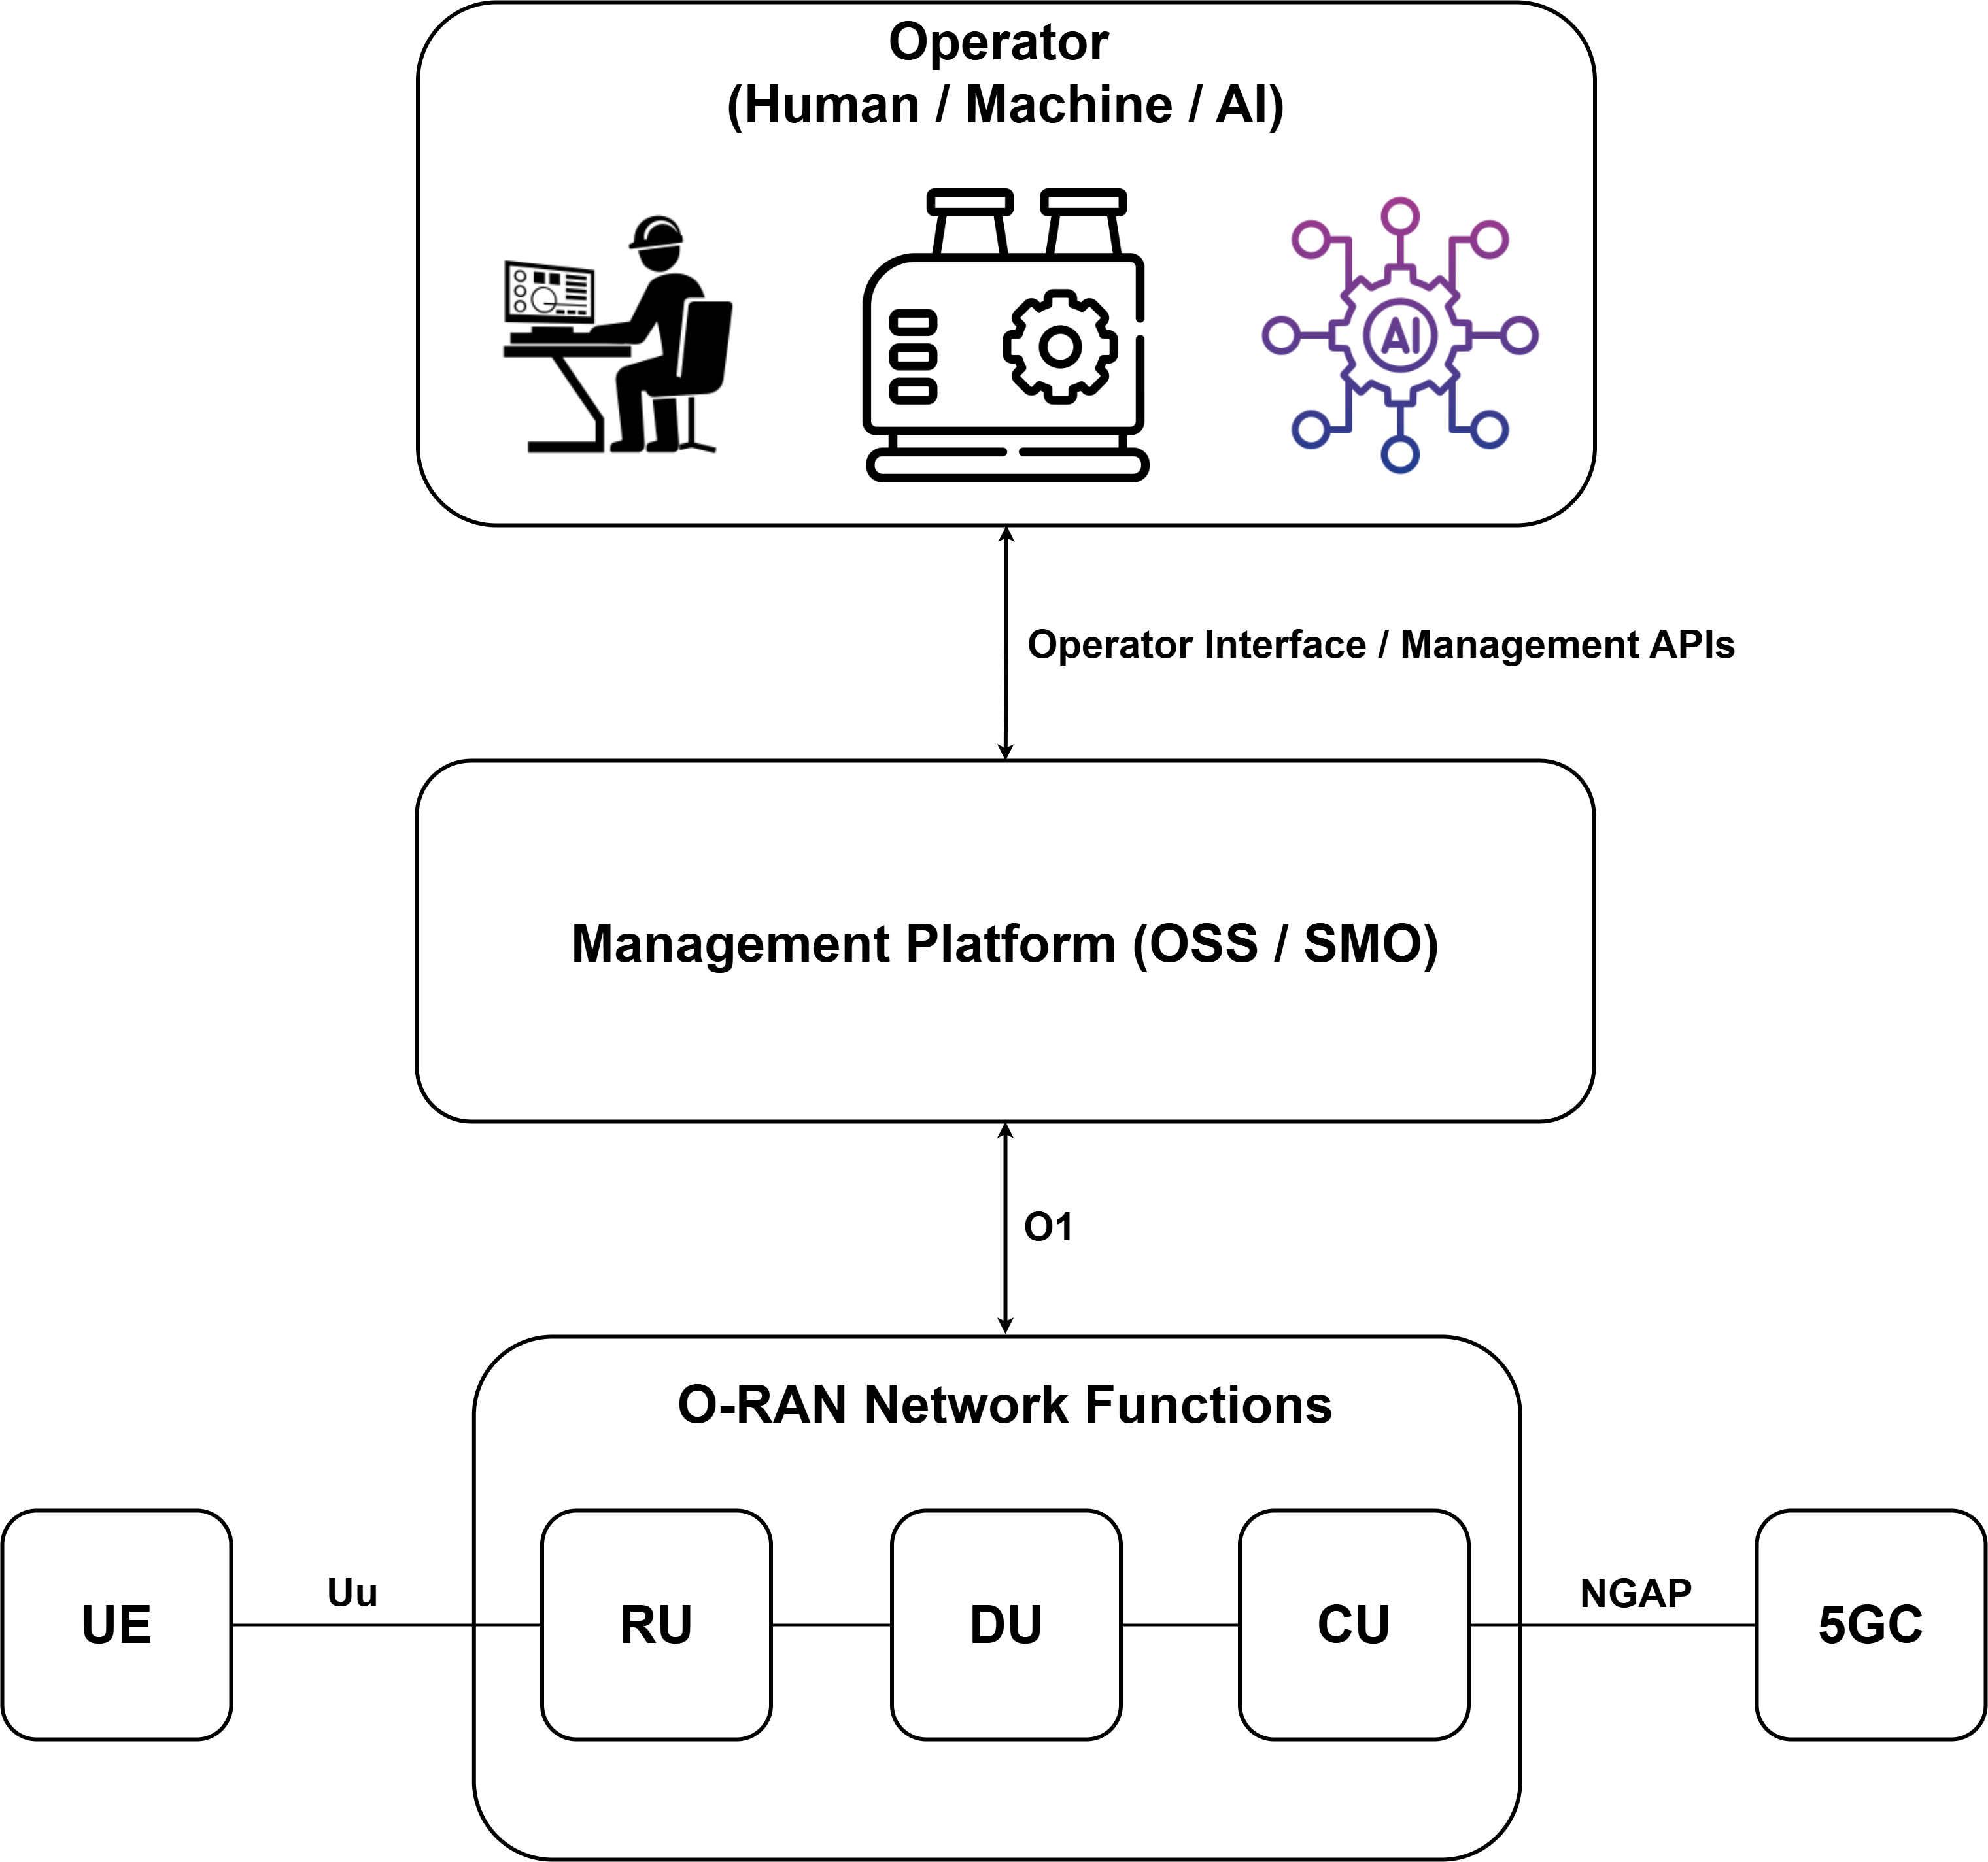
\includegraphics[width=1\linewidth]{figure/LLM-system_model_version_v6.drawio.png}
  \caption{System model}
  \label{model}
\end{figure}

Without loss of generality, we consider the simple case in which the operator analyzes error logs and recommends network configurations for the O-RAN network functions. In this paper, we use the following metrics \cite{} to evaluate the performance of the operator by considering both linguistic accuracy and operational results of the network.


\color{red}{
List the metrics and their definitions:
}


\color{black}
\section{LLM Reasoning Framework}\label{LLMReasoningFramework}
This paper presents an LLM reasoning framework 
that establishes a pipeline from error logs to reasoning traces for automatic gNB parameter adjustment. 
Fig.~\ref{LLM_reasoning_framework} illustrates the proposed framework, comprising three main components: synthetic data generation, supervised fine-tuning (SFT), and LLM.
The LLM implements a reasoning loop that provides reliable configuration recommendations and validation. We expect the LLM can automatically interpret event logs collected from gNB, infer root causes, and provide actionable recommendations for parameter adjustments. 
Synthetic data generation utilizes a reasoning loop to automatically generate a high-quality synthetic reasoning dataset by converting error event logs into structured reasoning traces and capturing causal relationships and decision-making processes. We utilize AI coding assistants to generate invalid configuration parameters and validate the root causes of these incorrect parameters through subsequent event logs collected from the RAN. We then develop an SFT pipeline to instill the domain-specific knowledge of network logs and gNB configurations obtained from the synthetic reasoning dataset into the LLM.

{\color{red} 
[Ray:]

1. ALL the blocks shown on the figure should be explained. On Fig. 1, you don't have to show the internal blocks of the Management Platform unless needed.

[Johnson:] Done

2. Please use the {\bf same term you used in the figure} to revise the text shown above. The terms of Error Log, Error conf, Base LLM, Fine-tuned LLM should be mentioned in the text.

3. Do you input Error Conf to AI Coding Assistant? Or, use AI Coding Assistant to generate Error Conf?

[Johnson] I input Workable configuration and use the AI Coding Assistant to mutate it into an Error Configuration through a Configuration Mutation Prompt.

4. Remove LLM from the AI Coding Assistant. It's NOT the same as the LLM you showed in the Supervised Fine-tuning block. 


For Figures:

5. How do you link your Figs. 2 to 3?

[Johnson]: I will remove the original Figs. 3

6. Please refer to the other paper to draw your figures. Figs. 2, 3, and 4 are NOT consistent.

7. From Fig. 1, the Operator DIDN't connect to RAN. Why do you show RAN on Fig. 5?


8. Please use the SAME term in the text, figure, and APPENDIX A. You should be able to identify the inconsistencies among figures before writing them down. Your figure should be based on your implementation.
For example, 

On Fig. 2, you showed that the 

- I/P to AI Coding Assistant is Error Log and Error Configuration files (Error Conf). 

- O/P is Reasoning Trace

On Fig. 4, 

- I/P to AI Coding Assistant becomes Configuration Mutation Prompt and Workable Configuration Files.

- O/P is Configuration Mutation Set

For APPENDIX A:

9. How does your prompt accurately generate synthetic data to represent rare or unusual events? How do you plan to prove it?

10. Is the 'COMPONENT' in APPENDIX A the same as the 'Component' in Table II?

[Johnson]: Only CU/DU/UE

11. What $N_VARIATIONS$ did you use? How can you ensure the AI Coding Assistant can produce distinct, unique test cases? 

[Johnson] I am currently using 25 as the quantity for $N_{VARIATIONS}$.

[Johnson] To ensure the AI Coding Assistant generates unique and diverse test cases, the LLM temperature is set to 1.This encourages stochastic sampling, allowing the model to explore multiple valid configurations instead of deterministic outputs.

12. How do you ensure the AI Coding Assistant can accurately determine the error categories (e.g., the valid range of a parameter)?

13. How/Where do you design Log Analysis and Reasoning?
} 


\begin{figure}[h]
    \centering
    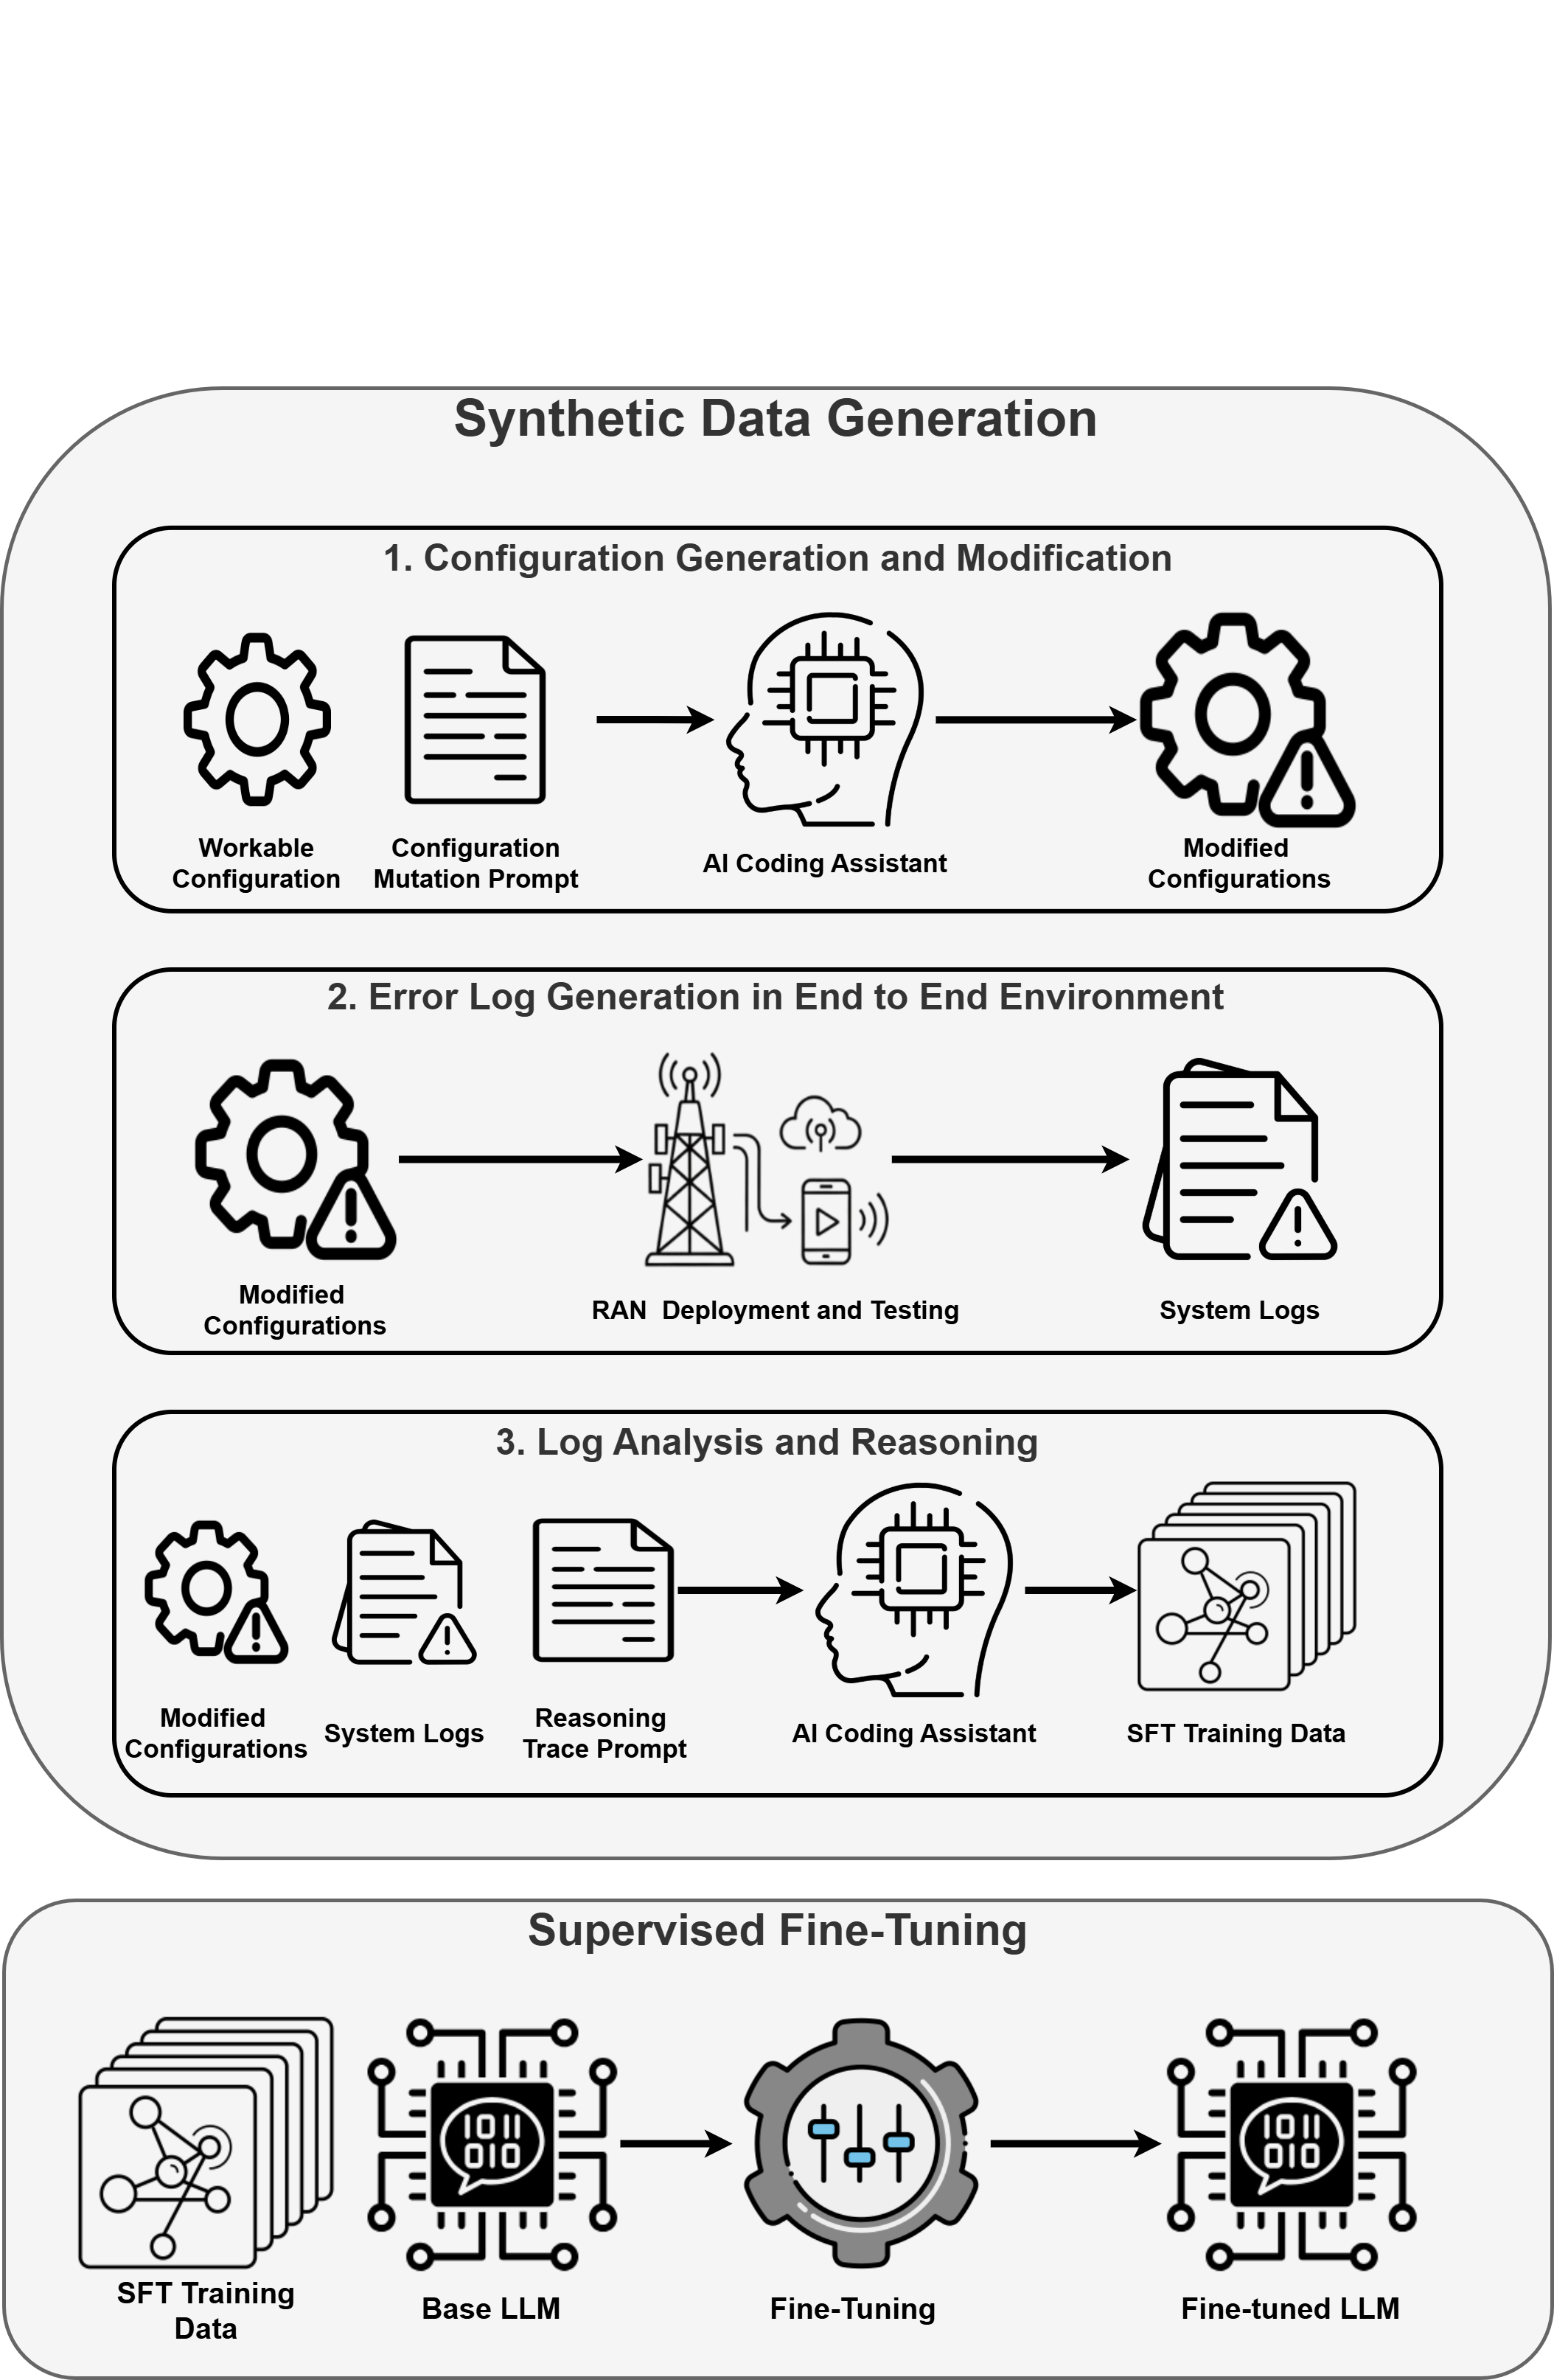
\includegraphics[width=1\linewidth]{figure/LLM-LLM Reasoning Framework_v2.drawio.png}
    \caption{LLM Reasoning Framework}
    \label{LLM_reasoning_framework}
\end{figure}
}

\subsection{Synthetic Data Generation}

\color{blue}{
To achieve this objective, this study designed a three-module pipeline (as shown in the Synthetic Data Generation block of Figure~\ref{LLM_reasoning_framework})

\begin{itemize}
    \item Modified Configuration Generation: This module is responsible for generating a large number of configuration files with different variations based on input configuration files, hereinafter referred to as Module-One.
    \item Error Log Generation in E2E Environment: This module is responsible for executing the configuration file generated by Module One on E2E testing platform and collecting the last 100 lines of log output from each system component (CU, DU, UE), hereinafter referred to as Module-Two.
    \item Log Analysis and Reasoning: This module is responsible for analyzing logs collected by Module-Two and using the Reasoning LLM to infer root causes of failures and erroneous parameters, hereafter referred to as Module-Three.
\end{itemize}
}



\subsubsection{Configuration Generation and Modification}

\color{blue}{
This step is used to generate a large number of configuration files. These generated configuration files will be used in the second phase of E2E testing and will produce log data.

\begin{itemize} 
    \item Workable Configuration - Under these settings, the UE can successfully establish a PDU session and obtain an IPv4 address when running the gNB. And these configuration files will serve as a baseline for the AI coding assistant to make modifications.
    \item Configuration Mutation Prompt - Instruct the AI coding assistant on how to create a configuration change set based on available configuration files, including the generated format, tools used, quantity generated, and target components. Users can adjust \texttt{COMPONENT} to select the network element to modify (CU, DU, or UE in this paper). Users can also adjust \texttt{N\_VARIATIONS} to control the number of errors generated (this paper recommends 25), see Appendix \ref{app:gen_prompt} for details.
\end{itemize}
}
\color{blue}{
Once workable configuration and configuration mutation prompt are entered, the AI coding assistant will generate the modified configuration according to the following process:
\begin{enumerate}
  \item Analyze input files - The AI coding assistant first analyzes the workable configuration content of the input and determines the parameters that can be modified and their types.
  \item Generate CMS - The AI coding assistant generates a Config Mutation Set (CMS) based on the understanding in step one. The key structure is shown in Table \ref{table:Definition_of_Config_Mutation_Set} , and the format is shown in output schema in the appendix \ref{app:gen_prompt}.
  \item Generate modified configuration - Based on the modified\_key and error\_value in the CMS generated in step two, modify the workable configuration to generate modified configuration.
\end{enumerate}
}



\color{blue}{
Traditional manual configuration modifications are not only extremely inefficient but also struggle to cover all possible error combinations. Common rule-based approaches also have limitations, often generating only a small number of fixed error patterns.For the SFT model, we need to exhaustively enumerate errors as much as possible. Therefore, in this phase, we have chosen to utilize the AI coding assistant to assist in generating. Moreover, in terms of generation methodology, directly outputting the entire configuration file consumes both tokens and time, especially when the configuration file is large. Longer contexts can easily cause weaker models to hallucinate, produce formatting errors, or generate garbled text. To avoid such situations, we also propose a partial generation approach that further improves efficiency and reduces the likelihood of LLM failures or errors when generating long texts.
}




\begin{table}[H]
    \centering
    \caption{Definition of Config Mutation Set}
    \label{table:Definition_of_Config_Mutation_Set}
    \begin{tabular}{|m{2.5cm}|m{5.5cm}|}
        \hline
        \textbf{Component} & \textbf{Definition and Purpose} \\
        \hline
        \texttt{filename} & Specifies the name of the base configuration file to which the modification should be applied. \\
        \hline
        \texttt{modified\_key} & Defines the hierarchical path (using JSON Path notation) to the specific parameter that needs to be altered. \\
        \hline
        \texttt{original\_value} & Records the value of the parameter as found in the initial, workable configuration file for verification. \\
        \hline
        \texttt{error\_value} & The new value that replaces the original value. This often represents an injected fault, a boundary case, or a required new setting. \\
        \hline
    \end{tabular}
\end{table}
\subsubsection{Error Log Generation in E2E Environment}
\color{blue}{
Once the gNB loads and executes the configuration file, it begins continuously outputting a large amount of logs to record detailed information such as system execution status, signaling handover processes, and the operational status of each channel. When gNB get issue, engineers typically analyze these logs to deduce the possible source of the problem. More experienced engineers are often able to identify the cause of the failure more quickly because different error scenarios leave representative error messages in the logs, and these messages are highly correlated with the configuration file currently in use.

This step uses the modified configurations generated during the configuration generation and modification stage as input for RAN deployment and testing. We used OAI RAN and OAI CN as the test platform for this paper. The component definitions and hardware used in the experiment are described in Tables \ref{table:oai_testing_environment} and \ref{table:oai_equiment}. On this test platform, we sequentially execute each modified configuration and record the logs (CU/DU/UE logs) generated by each component during E2E procedure at the gNB and UE. The detailed process is as follows:

\begin{enumerate}
    \item Launch the CU and start recording the CU execution log.
    \item Wait for 4 seconds to ensure the CU is fully initialized.
    \item Launch the DU and start recording the DU execution log.
    \item Wait for another 4 seconds to ensure the DU is fully initialized.
    \item Launch the UE and start recording the UE execution log.
    \item Keep the system running for 30 seconds to collect sufficient E2E log data.
    \item After data collection, extract the last 100 lines from each component's log and terminate all active processes.
\end{enumerate}

Finally, we will filter the logs. If there is no "received PDU session establishment accept" in the UE Log, we will consider it as a failure to establish a PDU session and retain it as an error log (e.g., gNB initialization failures, RRC establishment failures, NG Setup failures, and other issues that prevent the UE from successfully establishing a PDU session). These error logs will serve as input for the next stage, Log Analysis and Reasoning, to build the training data for SFT training.




\begin{table}[H]
    \centering
    \caption{Server Hardware Configuration}
    \label{table:oai_equiment}
    \begin{tabular}{ll}
    \hline
    \textbf{Item} & \textbf{Specification} \\
    \hline
    Server Model        & Dell PowerEdge R750 \\
    CPU Model           & Intel Xeon Gold 6326 \\
    Clock Frequency     & 2.90 GHz \\
    Logical CPU(s)      & 32 \\
    \hline
    \end{tabular}
\end{table}


\begin{table}[H]
    \centering
    \caption{Definition of the OAI Testing Environment Module}
    \label{table:oai_testing_environment}
    \begin{tabular}{|m{1.5cm}|m{6.5cm}|}
        \hline
        \textbf{Component} & \textbf{Definition and Purpose} \\
        \hline
        OAI CN & Contains multiple 5G core function elements, such as AMF, SMF, UPF, primarily responsible for user session management and data plane traffic processing. \\
        \hline
        OAI CU & Handles the RRC, SDAP, and PDCP functions within the 5G gNB protocols. \\
        \hline
        OAI DU & Handles the RLC and MAC functions of the 5G gNB, and features an integrated RF Simulator for emulating the radio environment. \\
        \hline
        OAI UE & Can establish connection and exchange data with the OAI network, used to simulate end-to-end connection scenarios. \\
        \hline
    \end{tabular}
\end{table}



\subsubsection{Log Analysis and Reasoning }
\color{blue}{For the design of the training data, this study assemble the data into four interrelated components:}
\color{blue}{
\begin{itemize}
    \item Current Network Component Log Snippet — Provides observations of fault events along with contextual information, such as base station logs, UE events, and packet statistics, allowing the model to identify abnormal patterns. Prior work\cite{rezaei2025fedllmguard} has shown that LLM can understand the semantics and context behind logs, enabling the detection of complex and evolving network anomalies.
    \item Current Network Component Configuration — Presents the complete set of system parameters, including but not limited to gNB settings, frequency bands, power levels, and antenna configurations, allowing the model to compare abnormal and normal configurations and identify potential root causes. The structured and comprehensive configuration data helps the LLM understand the network topology and operational status, providing a foundation for subsequent root cause analysis \cite{sana2025reasoning}.
    \item Misconfigured Parameter — Represents the specific configuration values that actually caused system faults, providing key evidence for the model to learn the causal mapping from misconfiguration to observed fault phenomena. Incorporating clearly labeled error samples in LLM diagnostic training significantly improves anomaly recognition and root cause analysis capabilities. When training data contains specific erroneous settings (e.g., incorrect SSB frequency, AMF/UPF IP, or improper compression algorithms), the model can learn the log features induced by these anomalies, understand their fault causes, and capture parameter-level diagnostic logic during SFT. According to \cite{sana2025reasoning}, models trained with structured error samples (including parameter identity, erroneous value, and causal reasoning trace) increased diagnostic accuracy from 18.85\% to 49.45\% highlighting the critical importance of precisely annotated misconfigurations for enhancing causal reasoning and fault diagnosis capabilities.
    \item Correct Parameter —
    % Serves as the target for generating remediation recommendations, guiding the LLM to learn causal reasoning from observed faults to corrective actions. Correct configurations are not only used to guide the generation of remediation suggestions but also serve as a reference for validating the effectiveness of model outputs, ensuring that proposed fixes are feasible and reliable in real network environments while avoiding model hallucinations. Network configurations are precise and deterministic—there is no concept of “approximately correct”; each parameter either functions properly or may cause a network fault. As noted in \cite{wang2024netconfeval}, introducing any imprecise target parameters in the training data immediately reduces model performance to 60–70\%. After fine-tuning, accuracy only recovers to over 95\% when the training dataset includes precise correct configurations. By combining correct and erroneous samples, the model can simultaneously learn fault causes and remediation logic, forming an end-to-end self-diagnosis and self-adjustment loop.
\end{itemize}
}


\subsection{Supervised Fine-tuning}

We use Supervise Fine Tuning 


% \section{Temp}
% {\color{red} Paragraphs put in the wrong sections will be moved here!}



% This research proposes a synthetic data generation workflow, as illustrated in Figure~\ref{Synthetic_data_generation_workflow}. 

% {\color{red} 
% Where is your AI coding Agent on Fig. 3? 

% Please refer to Appendix when you want to mention Configuration Mutation Prompt and Reasoning Trace "Generation??" Prompt?

% How do you generate 400 test cases using the prompt of "Produce {\bf{25}} distinct cases, covering different error categories."?

% On Fig. 3, you should remove everything for the RAN since the SMO is the only interface from Operator's perspective!
% }

% This three-module architecture forms a continuous and automated pipeline that bridges configuration manipulation, real network execution, and reasoning-based log interpretation. It not only ensures data consistency and technical fidelity but also allows scalable generation of high-quality reasoning traces for fine-tuning.

% \begin{figure}[h]
%     \centering
%     \includegraphics[width=1\linewidth]{figure/LLM-overview_v1.drawio.png}
%     \caption{Synthetic data generation workflow}
%     \label{Synthetic_data_generation_workflow}
% \end{figure}

% \color{blue}{
% In the overall process, the system first (Block 1) utilizes the LLM to automatically generate new and appropriately {\color{red}(definition is required!)} modified 5G Configurations based on an input prompt and a workable {\color{red}(definition is required!)} configuration file. Next (Block 2), these {\color{red}(what does "these" mean?)} configurations are deployed to the OAI $5\text{G}$ test platform, which includes components such as the OAI CN, OAI CU, OAI DU, and OAI UE, {\color{red}(Did you deploy configurations to all of them?)} for actual execution and functional verification. Finally (Block 3), the system collects the OAI operational logs {\color{red}(what is "operational log" mean?)}, which are then analyzed by the LLM to generate "Reasoning Traces". These reasoning traces will be organized into high-quality training data {\color{red}(HOW?)} for subsequent SFT of the LLM, enabling the model to gradually acquire the ability to understand and infer $5\text{G}$ network behavior, thereby improving its performance in the field of network automation.
% }





% ---------- Error Log Generation Architecture ----------
% \subsection{Synthetic Data Generation}

% Figure $\ref{Error_Log_Generation_Architecture}$ illustrates the error log generation architecture proposed in this study. 
% {\color{red}(Please describe ALL components shown on your figure!)}
% The primary objective of this system 
% {\color{red}(What is the "system"?)} 
% is to construct an efficient and controllable {\color{red}(How do you construct "efficient and controllable"?)} 
% experimental platform for systematically synthesizing fault data within the 5G 
% {\color{red}(Should we limit our work to 5G?)} 
% network environment. The architecture integrates the flexibility of $\text{LLMS}$ 
% {\color{red}(What is this?)} 
% in configuration mutation with the $\text{E2E}$ simulation capability of $\text{OAI}$, enabling automated generation 
% {\color{red}(Please write down HOW you "enable automated generation".)} 
% of high-quality test logs 
% {\color{red}(Please prove that how you generate "high-quality test logs".)} 
% with clearly defined root causes. 
% {\color{red}(Please show us how you get "clearly defined root causes".)} 
% This design not only replicates potential fault scenarios found in real-world network operations but also establishes a traceable and semantically aligned dataset for subsequent $\text{SFT}$ model training.
% {\color{red}(How can you prove it?)} 

% \begin{figure}[h]
%     \centering
%     \includegraphics[width=1\linewidth]{figure/error_log_gen.png}
%     \caption{Error Log Generation Architecture}
%     \label{Error_Log_Generation_Architecture}
% \end{figure}

% The overall workflow 
% {\color{red}(of What?)} 
% consists of three main stages. 
% {\color{red}(Where are the "three main stages"?)} 
% First, the system starts from a verified Workable Configuration File that ensures stable $\text{E2E}$ connectivity for the $\text{UE}$ within the $\text{OAI}$ environment, serving as a reliable experimental baseline. Second, a configuration mutation prompt is designed to guide the LLM 
% {\color{red}(We have AI coding assistant and LLM. Don't mix them up!)}
% in performing controlled variations, specifying the target components (e.g., CU, DU, UE), mutation strategies (e.g., parameter out-of-range, logical inconsistency, or syntax errors), and the desired diversity of generated samples. This allows the model to produce multiple Modified Configuration Files containing potential faults in a systematic and scalable manner. Third, the generated configurations are automatically deployed into the OAI E2E testbed—comprising the Core Network, CU, DU, and UE—and executed in batches through the RF Simulator. This process triggers a variety of fault scenarios such as gNB startup failure, cell search errors, random access issues, radio resource control (RRC) establishment failure, or NG interface handshake problems. Throughout each run, detailed protocol-level logs from CU, DU, and UE are continuously collected to capture precise timestamps, failure locations, and protocol symptoms. The resulting configuration–log paired dataset establishes explicit causal relationships between known configuration changes and observed system faults, forming a critical foundation for intelligent reasoning and supervised fine-tuning in subsequent model training.



% ----------  Reasoning-Trace Generation Architecture ----------
% \subsection{Reasoning Trace Extraction}


% After completion the automated generation of high-quality fault data, this study further proposes the reasoning trace generation architecture, as illustrated in Figure $\ref{Reasoning_Trace_Generation_Architecture}$. 
% {\color{red}(Please describe ALL components shown on your figure!)}
% The goal of this module is to automatically extract causal relationships and semantic representations from fault logs and their corresponding configuration files, generating coherent and interpretable reasoning traces that support knowledge construction and model training for automated debugging.

% \begin{figure}[h]
% \centering
% \includegraphics[width=0.9\linewidth]{figure/error_log_analyze.png}
%   \caption{Reasoning-Trace Generation Architecture.}
%   \label{Reasoning_Trace_Generation_Architecture}
% \end{figure}

% The system aligns and formats the CU, DU, and UE logs 
% {\color{red}Should we add the prompt for UE?} 
% along with their corresponding Modified Configuration Files from the OAI environment into a unified Defined Input Format (as shown in Table \ref{tab:DefinedInputFormat}). This format retains key elements related to root causes, including abnormal parameters {\color{red}(?)}, protocol error codes {\color{red}(?)}, and event sequences {\color{red}(?)}, providing the model with structured and semantically meaningful input data {\color{red}(?)}. 
% {\color{red}Please use the table to show us ho you do it! How do you choose the log?}

% Then, a Reasoning Trace Prompt (see Appendix \ref{app:reasoning_trace_prompt}) is designed to guide the LLM in generating reasoning traces for each fault case. The prompt template explicitly defines the output structure and logical hierarchy, allowing the model to consistently describe the complete causal chain from symptom observation to root-cause inference.
% {\color{red}Could we briefly summarize the design concept of the prompt? What is the main differences between DU and CU Config.?}

% Finally, the generated reasoning traces are systematically collected and organized as SFT training data, serving as high-quality exemplars that teach the model how to reason through fault diagnosis tasks in a structured and explainable manner.




\section{Experimental Results}\label{ExperimentalResults}
In this paper, we use Cursor \cite{cursor2025} and GitHub Copilot \cite{copilot2025} to build the pipeline and create error logs and reasoning traces.

\section{Conclusions}\label{Conclusions}



% ---------- References (BibTeX) ----------
\bibliographystyle{IEEEtran}
\bibliography{reference}



% ---------- appendix----------
\onecolumn
\clearpage 
\appendices        
% =============================================
% 文件名: appendix.tex
% 描述: 包含附录内容,包括 Fuzz Test Prompt 的定义
% =============================================

% 确保在 main.tex 中正确加载了 tcolorbox 和 listings 宏包

\section{Configuration Mutation Prompt}
\label{app:gen_prompt}
\begin{tcolorbox}[
    % ... (其他样式)
    box align=center,
    width=\textwidth,
    colback=white,
    colframe=black,
    arc=3mm,
    fonttitle=\bfseries\color{white},
    colbacktitle=black,
]
Here is the task: You are a 5G gNB configuration fuzz-test expert specializing in the \textbf{\{COMPONENT\}} component.
Given the following valid JSON configuration (Reference JSON) and the original .conf (Baseline Conf), generate exactly \textbf{\{N\_VARIATIONS\}} single-key error test cases and output them as a JSON array.

\vspace{0.5em}\hrule\vspace{0.5em}

\textbf{Rules for Error Generation}
\begin{itemize}
    \item[1.] Single Modification: Modify exactly one key per test case (a single-key error).
    \item[2.] Quantity: Produce \textbf{\{N\_VARIATIONS\}} distinct, unique test cases.
    \item[3.] Realism: Errors must be realistic and likely to cause system faults, configuration rejection, or unexpected behavior in a gNB \textbf{\{COMPONENT\}} system.
    \item[4.] Format Adherence: Your output MUST be a JSON array following the "Output Schema" structure.
    \item[5.] Clean Output: Your entire response MUST be only the JSON array. Do not include any other text, explanations, or code blocks outside the final JSON.
    \item[6.] Error categories (cover at least these):
    \begin{itemize}
        \item out\_of\_range
        \item wrong\_type
        \item invalid\_enum
        \item invalid\_format
        \item logical\_contradiction
        \item missing\_value
    \end{itemize}
\end{itemize}

\vspace{0.5em}\hrule\vspace{0.5em}

\textbf{Input: Workable .conf file content (for context)}
\begin{verbatim}
---[START {COMPONENT}.CONF]---
{conf_content}
---[END {COMPONENT}.CONF]---
\end{verbatim}

\vspace{0.5em}\hrule\vspace{0.5em}

\textbf{Input: Reference .json file content (The base configuration to modify)}
\begin{verbatim}
---[START {COMPONENT}.JSON]---
{json_content}
---[END {COMPONENT}.JSON]---
\end{verbatim}

\vspace{0.5em}\hrule\vspace{0.5em}

\textbf{Output Schema (Produce a JSON array of objects like this)}
\begin{verbatim}
[
    {
      "filename": "{COMPONENT}_case_001.json",
      "modified_key": "path.to.the.key",
      "original_value": "original_value_from_json",
      "error_value": "new_generated_error_value"
    },
    // ... Repeat for N_VARIATIONS
    {
      "filename": "{COMPONENT}_case_{N_VARIATIONS}.json",
      "modified_key": "path.to.the.key",
      "original_value": "original_value_from_json",
      "error_value": "new_generated_error_value"
    }
]
\end{verbatim}

\vspace{0.5em}\hrule\vspace{0.5em}

Generate the \{N\_VARIATIONS\} \{COMPONENT\} error-case variations now as a JSON array.
\end{tcolorbox}


% ==============================================
% File: 5G_NR_OAI_Reasoning_Trace_Prompt.tex
% Description: LaTeX-formatted prompt for 5G NR / OAI Reasoning Trace Generation
% ==============================================


\section{Reasoning Trace Prompt}
\label{app:reasoning_prompt}
\begin{tcolorbox}[
    % ... (其他样式)
    box align=center,
    width=\textwidth,
    colback=white,
    colframe=black,
    arc=3mm,
    fonttitle=\bfseries\color{white},
    colbacktitle=black,
]

You are an expert 5G NR and OpenAirInterface (OAI) analyst. Your task is to analyze the provided JSON containing logs from CU, DU, and UE (for the error case), the misconfigured parameter causing the issue, and the extracted network configuration (focused on gnb.conf and ue.conf parameters as JSON objects), to generate a detailed step-by-step reasoning trace. This trace diagnoses the issue, identifies the root cause based on the misconfigured parameter, and explains the fix. The reasoning should be structured to teach another model how to perform similar analysis, emphasizing systematic thinking, cross-component correlation, and use of external knowledge via tools if needed. Assume advance knowledge of the issue from the misconfigured parameter to guide the diagnosis.

\vspace{1em}

Input JSON structure:
\begin{itemize}
    \item[\textbullet] \textbf{"misconfigured\_param"}: The wrong parameter value causing the issue (e.g., \texttt{"prach\_config\_index=64"}).
    \item[\textbullet] \textbf{"correct\_param"}: The correct parameter value in workable configuration (e.g., \texttt{"prach\_config\_index=98"}).
    \item[\textbullet] \textbf{"logs"}: Object with \texttt{"CU"}, \texttt{"DU"}, \texttt{"UE"} arrays of log lines for the error case.
    \item[\textbullet] \textbf{"network\_config"}: Extracted configuration as a JSON object with \texttt{"gnb\_conf"} and \texttt{"ue\_conf"} subsections (e.g., \texttt{gnb\_conf} includes parameters like \texttt{prach\_config\_index}, \texttt{tdd\_ul\_dl\_configuration\_common}; \texttt{ue\_conf} includes \texttt{imsi}, \texttt{frequency}). Parse it fully, extract relevant parameters, and use for mismatches with logs and \texttt{misconfigured\_param}.
\end{itemize}

\vspace{1em}

Think step by step, writing down all thoughts as you go, guided by the \texttt{misconfigured\_param} for accurate diagnosis. Follow this structure in your response:
\begin{enumerate}[1.]
    \item \textbf{Overall Context and Setup Assumptions}\\
    Summarize the scenario (e.g., OAI SA mode with \texttt{--rfsim --sa} options), expected flow (e.g., component init $\rightarrow$ F1/NGAP setup $\rightarrow$ UE connection/PRACH $\rightarrow$ RRC/PDU session), and potential issues to look for (e.g., config mismatches in PRACH or SIB encoding, asserts in code, connection failures).\\
    Parse \texttt{network\_config}'s \texttt{gnb\_conf} and \texttt{ue\_conf}, summarize key parameters (e.g., \texttt{prach\_config\_index} in \texttt{gnb\_conf}), and note initial mismatches with logs or \texttt{misconfigured\_param}.
    
    \vspace{1em}
    \item \textbf{Analyzing CU Logs}\\
    Break down initialization (e.g., mode confirmation, threads, GTPU/NGAP setup), key events (e.g., AMF connection, F1AP start), and anomalies (e.g., incomplete logs or stalled states). Cross-reference with \texttt{network\_config}'s \texttt{gnb\_conf} where relevant (e.g., AMF IP or GTPU ports).
    
    \vspace{1em}
    \item \textbf{Analyzing DU Logs}\\
    Focus on PHY/MAC errors (e.g., PRACH config issues, assertions such as ``bad r: L\_ra 139, NCS 209''). Break down initialization (e.g., antenna ports, TDD period), identify crash points, and link findings to \texttt{network\_config}'s \texttt{gnb\_conf} parameters like \texttt{prach\_config\_index}.
    
    \vspace{1em}
    \item \textbf{Analyzing UE Logs}\\
    Focus on connection attempts (e.g., repeated connect failures to rfsim server). Link observed UE behavior to \texttt{network\_config}'s \texttt{ue\_conf} parameters such as \texttt{frequency} or \texttt{rfsimulator\_serveraddr}.
    
    \vspace{1em}
    \item \textbf{Cross-Component Correlations and Root Cause Hypothesis}\\
    Correlate timelines (e.g., DU crash prevents rfsim server, causing UE connect fails; CU waits for DU). Use the \texttt{misconfigured\_param} for clues (e.g., known invalid \texttt{prach\_config\_index=64} causing ASN.1 failures). If uncertain about specification details, perform a web search with queries like ``3GPP TS 38.331 prach-ConfigurationIndex range'' or ``OpenAirInterface NR prach\_config\_index validation''. Hypothesize how specific \texttt{network\_config} entries (from \texttt{gnb\_conf}/\texttt{ue\_conf}) produce the observed issues, guided by the \texttt{misconfigured\_param}.
    
    \vspace{1em}
    \item \textbf{Recommendations for Fix and Further Analysis}\\
    Suggest configuration changes (e.g., set \texttt{prach\_config\_index} to a valid value), debugging steps, and tools to use. Output corrected \texttt{gnb.conf} and \texttt{ue.conf} snippets as JSON objects within the \texttt{network\_config} structure, and include brief comments explaining each change and why it fixes the issue.
    
    \vspace{1em}
    \item \textbf{Limitations}\\
    Note truncated logs, missing timestamps, or incomplete JSON inputs. If using external tools, call them before finalizing the root cause (for example via a function call placeholder like \verb|<xai:function_call>|). Base hypotheses on 3GPP specs (e.g., TS 38.211 for PRACH) and typical OAI code patterns, while incorporating the advance knowledge implied by the \texttt{misconfigured\_param}.\\
    \textbf{Important: Output only the reasoning trace.}
\end{enumerate}


\end{tcolorbox}



\end{document}
